\section{Supplementary Material 1 for Chapter \ref{ch:modcell2}} \label{apx:sm1-modcell2}

%\counterwithin{figure}{section}

\newcommand{\hbAppendixPrefix}{A}
%
\renewcommand{\thefigure}{\hbAppendixPrefix\arabic{figure}}
\setcounter{figure}{0}
\renewcommand{\thetable}{\hbAppendixPrefix\arabic{table}}
\setcounter{table}{0}
\renewcommand{\theequation}{\hbAppendixPrefix\arabic{equation}}
\setcounter{equation}{0}

\begin{figure}[h]
  \centering
  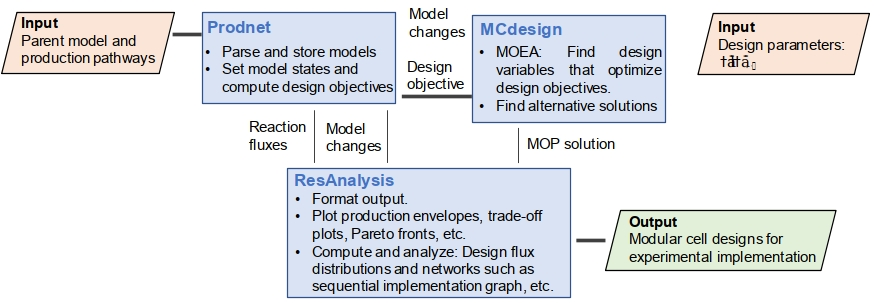
\includegraphics[width=\textwidth]{ms1-sf1}
    \caption[Software architecture of ModCell2]{Software architecture of ModCell2. The Prodnet class preprocesses production network models and computes design objectives. The MCdesign class serves as an interface between the MOEA optimization method and metabolic models. The ResAnalysis class loads the Pareto set computed by MCdesign and performs analyses to identify the most promising designs.}
\end{figure}

\begin{figure}[h]
  \centering
  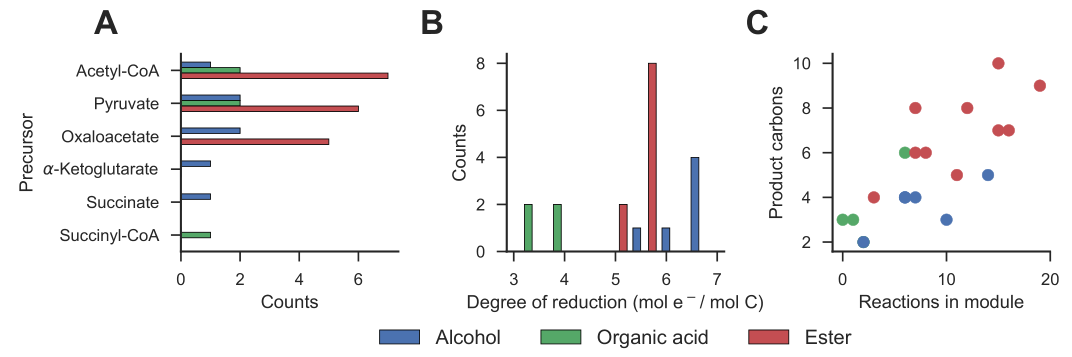
\includegraphics[width=\textwidth]{ms1-sf2}
    \caption[Biochemical properties of production modules]{Properties of 20 production modules used in the E. coli genome-scale metabolic model for biosynthesis of 6 alcohols, 4 organic acids, and 10 esters. (A) Distribution of precursor metabolites. (B) Distribution of degrees of reduction of target products. (C) Correlation between the number of product carbons and the number of reactions in production modules. Alcohols include ethanol, propanol, butanol, isobutanol, pentanol, and 1,4-butandiol; acids include pyruvate, D-lactate, acetate, and adipic acid; and esters include ethyl acetate, propyl acetate, isobutyl acetate, ethyl butanoate, propyl butanoate, butyl butanoate, isobutyl butanoate, ethyl pentanoate, isobutyl pentanoate, and pentyl pentanoate.
    }
\end{figure}

\begin{figure}[h]
  \centering
  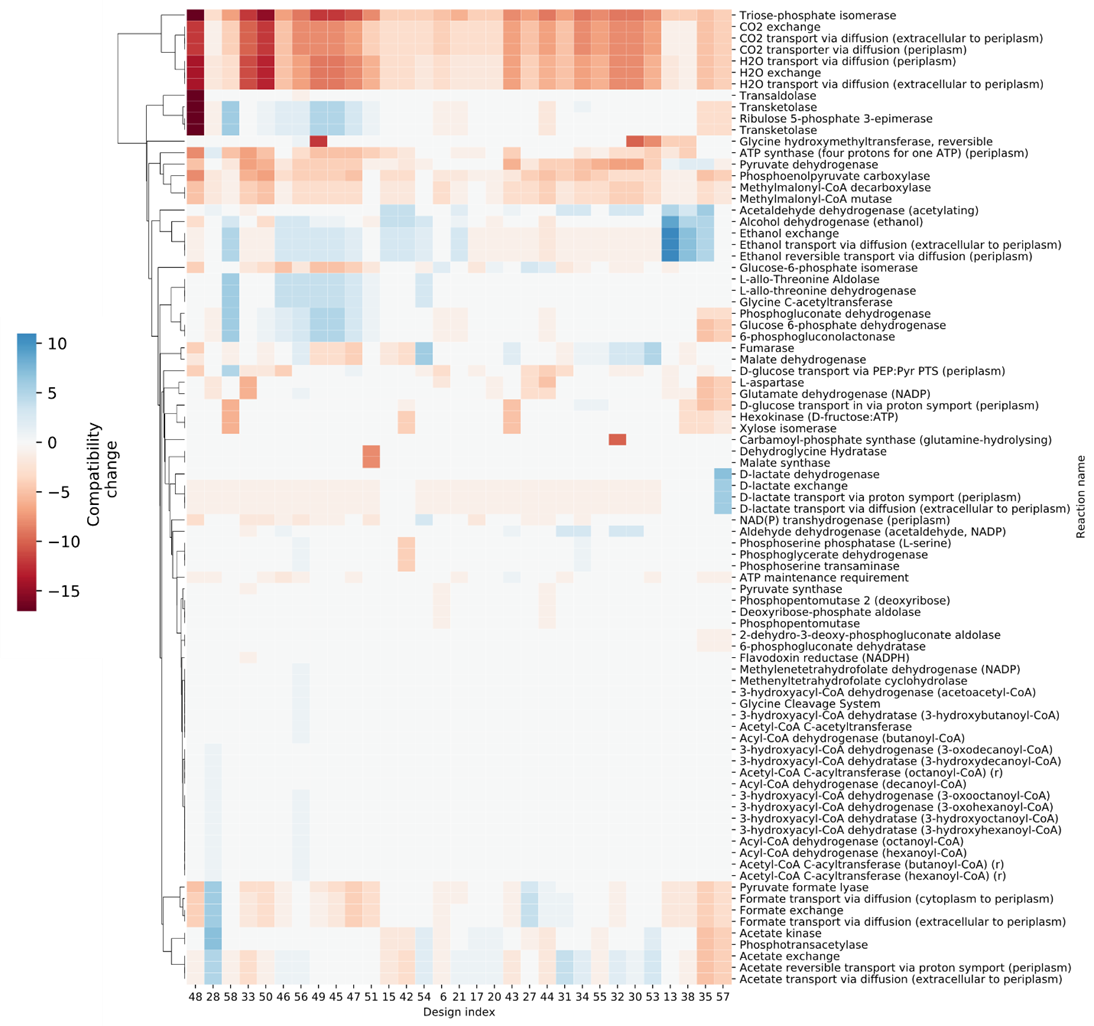
\includegraphics[width=\textwidth]{ms1-sf3}
    \caption[Robustness analysis of designs]{Robustness analysis for wGCP-4-0 designs for the E. coli genome scale model. Only the designs that are compatible with 4 or more products (compatibility  4) were considered. Each column corresponds to a design whereas each row corresponds to a single-reaction deletion. Included in the heat map are all reaction deletions with a compatibility change that is not 0 in at least one product.
    }
\end{figure}

\begin{figure}[h]
  \centering
  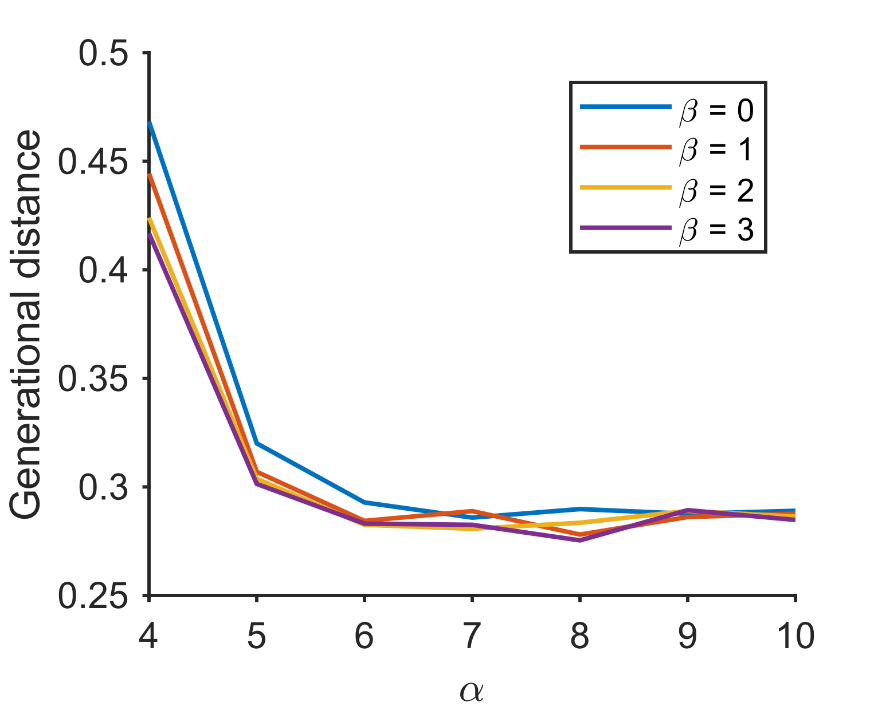
\includegraphics[width=.5\textwidth]{ms1-sf4}
    \caption[Generational distance among different design parameters]{Generational distances between the calculated Pareto fronts and the reference utopia point. The generational distance is calculated as follows: $GD=\frac{\left|d\right|_2}{\left|d\right|_1}$where  $d_j=\left| \PF^j - \PFs \right|_2$ where $\PF$ is the calculated pareto front and $\PFs=\vec{1}$ is the utopia point. A smaller value of $\mathit{GD}$ indicates the overall objective values in the Pareto front are closer to the utopia point. The calculation was performed for the iML1515 model with 20 products using the wGCP objective, various  and  values, and a run time of 10 h for all cases.
    }
\end{figure}
